%\subsection{Normalisation Using Beads: Accounting for Non-Biological Variation Across Samples}

The objective of flow cytometry is to capture variation in the biological sample not variation linked to the instrument or to other experimental factors.
Normalisation is the process of factoring out non-biological for sensible comparison fo samples analysed at different times or on different instruments.
In flow cytometry, one method of normalising fluorescence intensity is to convert Mean Fluorescence Intensity (MFI)
to Molecules of Equivalent Fluorochrome (MEF) \citep{Schwartz:1996jj,Dendrou:2009bl}.
In order to apply this conversion, specially designed beads of known and (assumed) constant fluorescence defined in terms of MEF are used as a reference.
The MEF property of these beads is deemed stable whereas the MFI of the bead population is dependent on the instrument and varies over time.

In our case, the beads used are specially manufactured so that they belong to six distinct populations of increasing MEF as shown in Table~\ref{table:fluorospheres}.
Following the bead manufacturer's guidelines, plotting the $\log_{10}(MEF)$ of these six bead populations against
the corresponding calculated $log_{10}(MFI)$ from the gated bead populations, we fit the linear regression:

\begin{equation}
    \log_{10}(\text{MEF})=\beta  \times \log_{10}(\text{MFI}) + \alpha
\label{equ:MEF}
\end{equation}

The MEF can then be obtained and is in fact a power transform of the MFI\footnote{This transform is only defined for strictly positive MFI values}:

%\[
%    MEF= 10^{\beta  \times log_{10}(MFI) + \alpha}
%]

\[
    \text{MEF}= 10^\alpha \times \text{MFI}^\beta
\]

%and so is only defined for 
%positive MFI values because $\beta$ is not an integer.

%If we add a location parameter $b$ then as expected the MEF does not scale linearly.
%\[
    %MEF= 10^\alpha \times (MFI+b)^\beta
%\]

The original MEF transform used by \citet{Dendrou:2009bl} assumes that $\beta=1$ which
gives similar results given that I found that the $\beta$ term in Equation~\ref{equ:MEF} turns out to be on average $0.96$.


In estimating the parameters $\beta$ and $\alpha$ of the linear model, only the non blank beads are used because the MEF of the blank beads is not specified by the manufacturer.
In fact extrapolating the MEF of the blank beads yields the detection threshold (Figure~\ref{figure:mef}) which we will see can be used in defining positive cell subsets.
The MEF of the blank beads is always greater than the intercept $\alpha$  which represents the log offset (the zero channel value).
%Below this threshold the intensity is meaningless as the blank beads contain by design no fluorochrome.

Typically even bead data is gated manually.
Here, in order to obtain $\beta$ and $\alpha$ parameters of the MEF transform, I will use an automatic process to gate the beads.

\begin{table} [hb]
\begin{center}
\begin{tabular} {|c c c c c c|}
\cline{1-6}
Population & FITC & RPE & REP-Cy5 & \textbf{APC} & PE-Texas Red\\
\cline{1-6}
1 & B & B & B & \textbf{B} & B \\
2 & 2,500 & 1,500 & 750 & \textbf{4,100} & 552\\
3 & 6,500 & 4,400 & 2,100 & \textbf{10,300} & 2,014\\
4 & 19,000 & 14,500 & 6900 & \textbf{25,500} & 6,975\\
5 & 55,000 & 43,800 & 22,100 & \textbf{67,300} & 20,685\\
6 & 150,000 & 131,200 & 77,100 & \textbf{139,100} & 71,888\\
\cline{1-6}
\end{tabular}
\end{center}
\caption{ \label{table:fluorospheres} FluoroSpheres from DakoCytomation. 
    The Molecules of Equivalent Fluorochromes (MEF) values for the six bead populations as provided by the manufacturer.
    B denote the blank beads which by design contain no fluorochrome.
    Of the six fluorochromes contained by each bead only APC is used in the experiment.
 }
\end{table}

\begin{figure}[hb]
    \centering
    \includegraphics[scale=0.6]{IL2RA/figures/BeadNormalisation/MEF.pdf}
    \caption{ Linear regression of bead MFI against MEF. The horizontal dash lines represent the MEF of the six bead populations.
    The red and green vertical lines define the range of memory CD25 MFI across all samples in \citet{Dendrou:2009dv}. }
    \label{figure:mef}
\end{figure}



Because all beads are known to be of identical shape and size, we expect a single cluster in the scatter channels.
Events which lie away from the main bead population are deemed to be beads clumped together or debris and so are discarded.
Once we have identified the main bead population we known that the beads belong to six populations distinguishable in the APC channel.

%We will see that these two steps are easily automated using existing tools (FlowClust on the scatter and K-Medoids on the APC channel)
%which implies that gating of bead data can be fully automated.
%Which in turn implies that channel normalisation using beads no longer needs to be a manual process.

\subsection{Bivariate Gating on Forward and Side Scatter}

%% Gating
% Scatter plots
\begin{figure}[ht]
%\begin{center}
    \begin{subfigure}[b]{.5\textwidth}
        \centering
        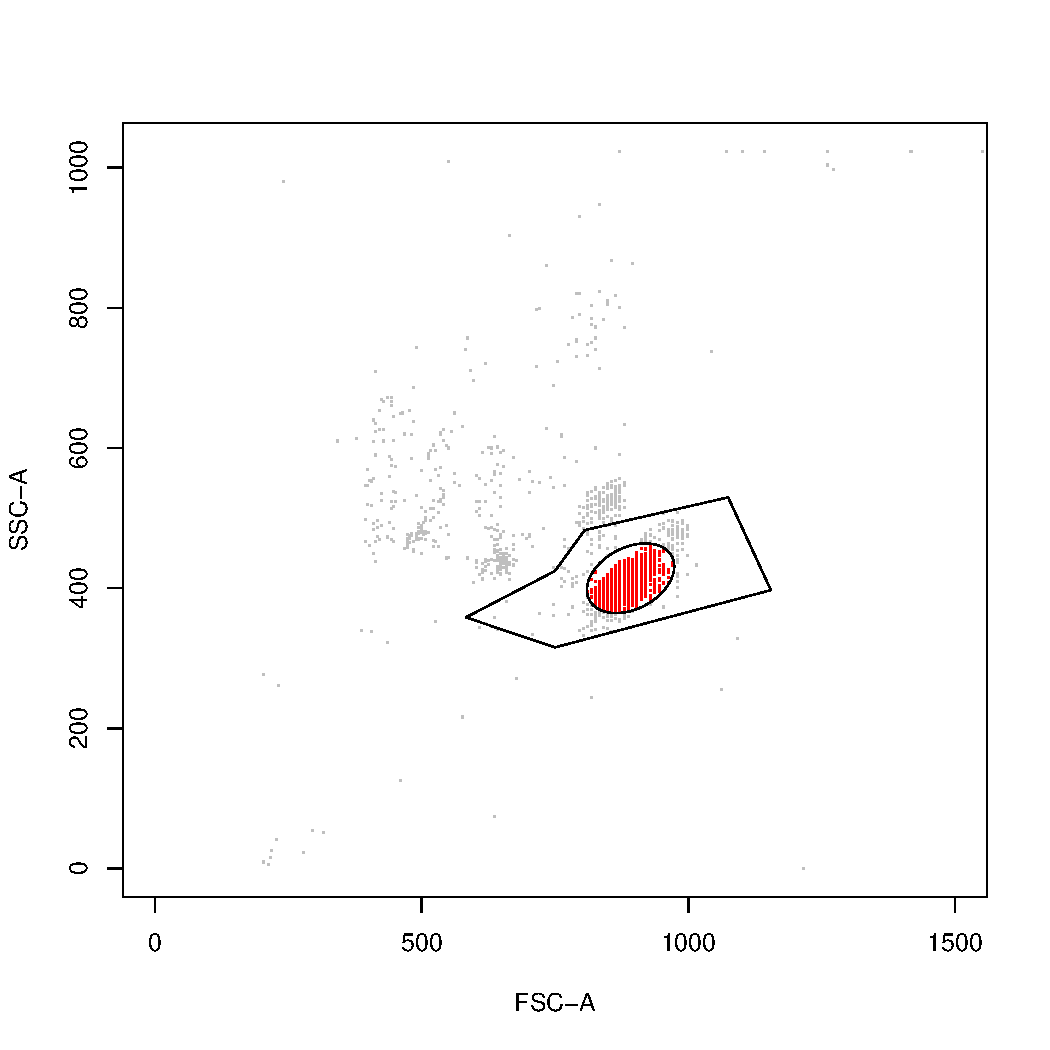
\includegraphics[scale=.5]{IL2RA/figures/Beads/manual-flowclust-scatter-gate-cad57.pdf} 
        \caption{Manual and FlowClust gating on scatter.}
    \end{subfigure}
    ~
    \begin{subfigure}[b]{.5\textwidth}
        \centering
        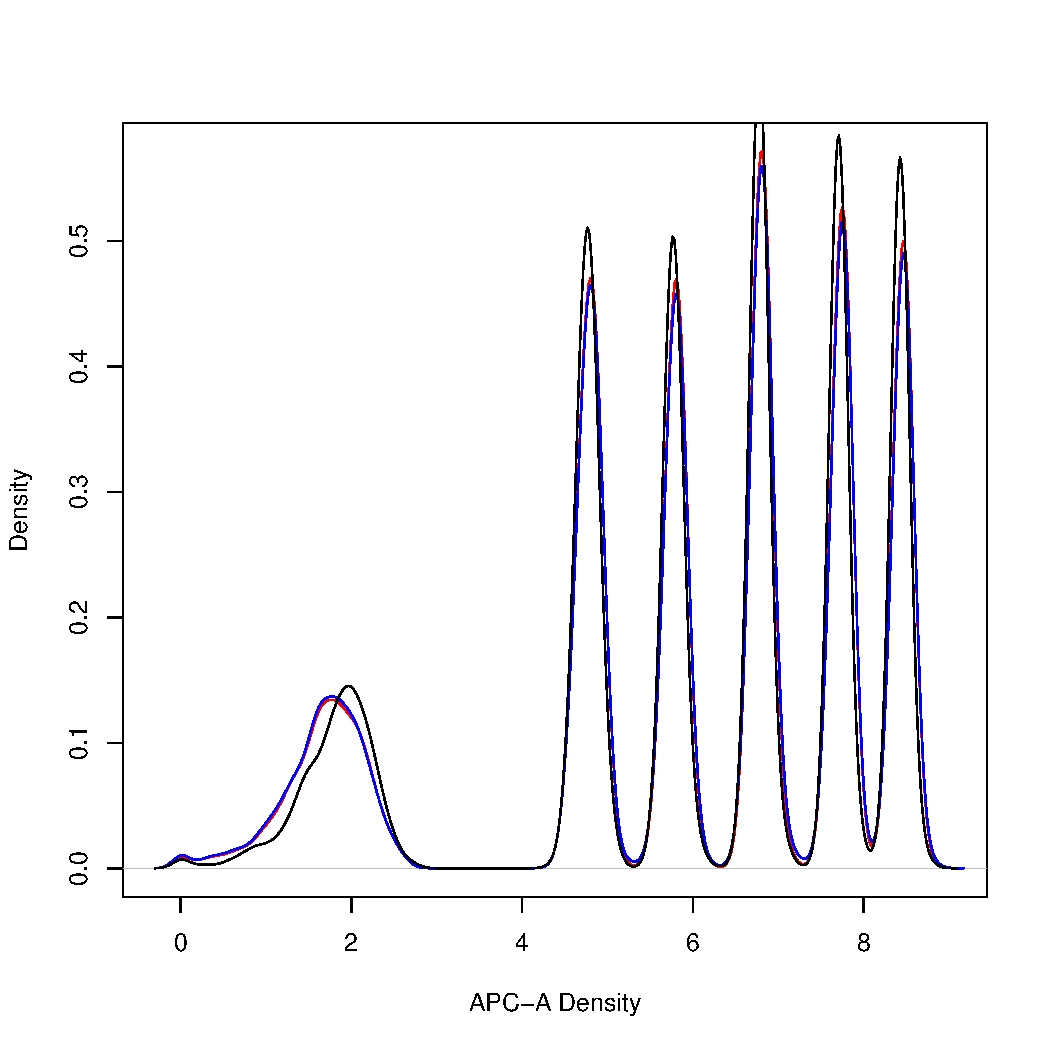
\includegraphics[scale=.5]{IL2RA/figures/Beads/manual-flowclust-apc-cad57.pdf} 
        \caption{density of $log$ APC after applying scatter gate.}
    \end{subfigure}
%\end{center}
\caption{ \label{figure:bead-gate}
  In Figure a), the gate applied by FlowClust (in red) is a subset of the gate applied through manual gating (in blue).
In Figure b) we notice that the effect of the scatter gating on the APC channel is to reduce the intensity of the first peak (the blank beads) and slightly increase the intensity of the other peaks.
Overall both manual and FlowClust gating seem to yield very similar distributions. }
\end{figure}



I first gated on both the forward and side scatter using \texttt{FlowClust} \citep{Lo:2008it}
to distinguish single beads from groups of beads which might go through the flow cytometer clumped together (Figure~\ref{figure:bead-gate}).
FlowClust proceeds by doing a Box-Cox transform to normalise the data, then fits a mixture of Student t-distributions
using the EM algorithm \citep{Dempster:1977ul}. In this case, there is a single populations as all beads are the same size.
%(Appendix~\ref{EM}).
%To filter out the predominant population of single beads, I fitted a single bivariate Student t-distribution on the two scatter dimensions (side and forward)\footnote{In this case, given we know that the number of clusters $K=1$ an even simpler way would be to use a single bivariate Gaussian.}.


\subsection{Univariate Gating on APC Channel}

Having gated the singlets, I subset the data and proceed to gate on the fluorescence channels to identify the six bead populations.
Since the bead population are distinguishable on all five fluorochromes (Table~\ref{table:fluorospheres}) it was first considered to use flowMeans to gate on all five fluorescent channels at the same time \citep{Aghaeepour:2010fv}.
However since we are solely interested in the APC channel, it was decided better to adhere to the bead manufacter's protocol (see Fluorospheres reference manual) of only gating on the channel of interest (APC channel).
Furthermore the detectors on the flow cytometer on which the beads were run are not properly calibrated for the other fluorochromes and so the signal is noisy which adds variance to the APC signal.
%However as FlowMeans is not capable of gating on only one dimension given that the number of cluster K is known and that the bead data is quite clean, more fundamental clustering alternatives were sought.
Given that the number of clusters K is known and that the bead data is quite clean, I tried two alternative clustering algorithms:

\paragraph{K-Means}

I first tried the K-means algorithm, in the one-dimensional case.
In K-means we try to minimise the overall sum of within-cluster sum of squares:

\[
    \sum_{k=1}^{K} \sum_{\mathbf x_i \in S_k} ( \mathbf x_i - \boldsymbol\mu_k )^2 ; \quad \boldsymbol\mu_k=\text{E}(x_i| x_i \in S_k)
\]

An alternative notation which helps parameterise the problem is to define the $N$ by $K$ matrix $\mathbf Z$ of responsibilities:

\[
\mathbf Z_{i,k} =
 \begin{pmatrix}
  1 & 0 & \cdots & 0 \\
  0 & 0 & \cdots & 1 \\
  \vdots  & \vdots  & \ddots & \vdots  \\
  0 & 1 & \cdots & 0
 \end{pmatrix}
\]

Then the overall sum of within-cluster sum of squares can be rewritten as:

\[
  \sum_{i=1}^N \sum_{k=1}^{K} ( x_i z_{ik} - \operatorname{E}(x_i z_{ik}) )^2 
\]

Further, if each cluster is scaled by its size then this can by rewritten in the one-dimensional case as:


\[
  \sum_{k=1}^{K} \operatorname{VAR}(\mathbf Z_k \mathbf X)
\]



The algorithm starts by picking K random points which are the initial guess as to where the cluster means lie.
Then for each iteration:
\begin{itemize}
    \item Each point $x_i$ is assigned to the cluster $S_k$ of the closest current cluster mean $\mu_k$.
    \item Based on this new cluster assignment, the new cluster mean of each cluster is computed.
\end{itemize}
The algorithm terminates when no cluster mean changes.

\vspace{1em}
\noindent


\paragraph{K-medoids}

In K-medoids instead of using the cluster means, we use the cluster medoids.
The medoid is defined as the point of the cluster which minimises the overall distance to all other points belonging to that cluster.

\[
    \sum_{k=1}^{K} \sum_{\mathbf x_i \in S_k} ( \mathbf x_i - \boldsymbol M_k )^2 ; \quad \boldsymbol M_k=\text{Medoid}(x_i| x_i \in S_k)
\]

The algorithm starts by picking K starting points which belong to the set of data points which are the initial guess as to where the cluster medoids lie.
Then for each iteration:
\begin{itemize}
    \item Each point $x_i$ is assigned to the cluster $S_k$ of the current closest cluster medoid $M_k$.
    \item Based on this new cluster assignment, the new cluster medoid of each cluster is selected.
\end{itemize}
The algorithm terminates when no cluster medoid changes.

\subsection{Normalisation}

The purpose of bead normalisation is to make intensity data comparable across days. 

\begin{figure}[ht]
%\begin{center}
    \begin{subfigure}[b]{.5\textwidth}
        \centering
        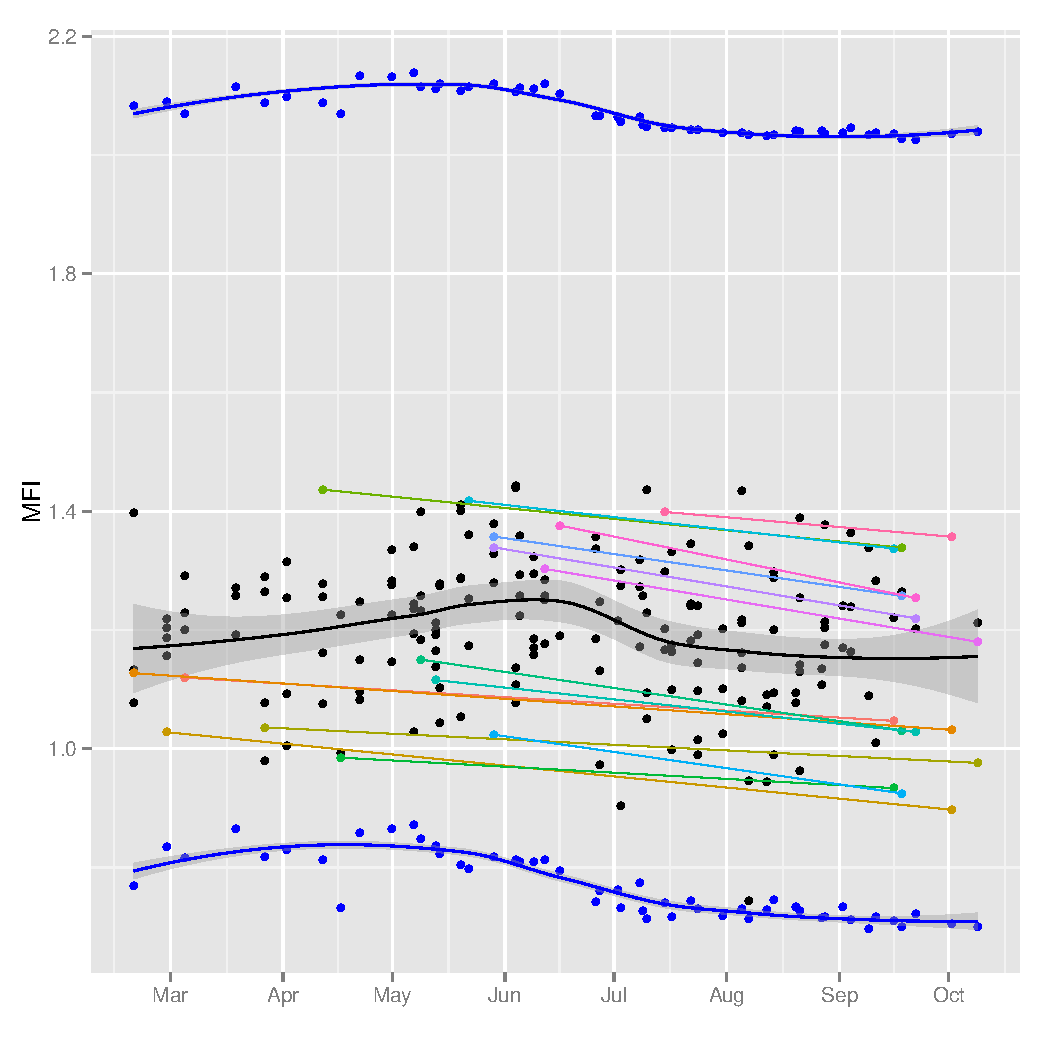
\includegraphics[scale=.5]{IL2RA/figures/CD25-MFI-time-effect-repeatability.pdf}
        \caption{Unormalised.}
    \end{subfigure}
    ~
    \begin{subfigure}[b]{.5\textwidth}
        \centering
        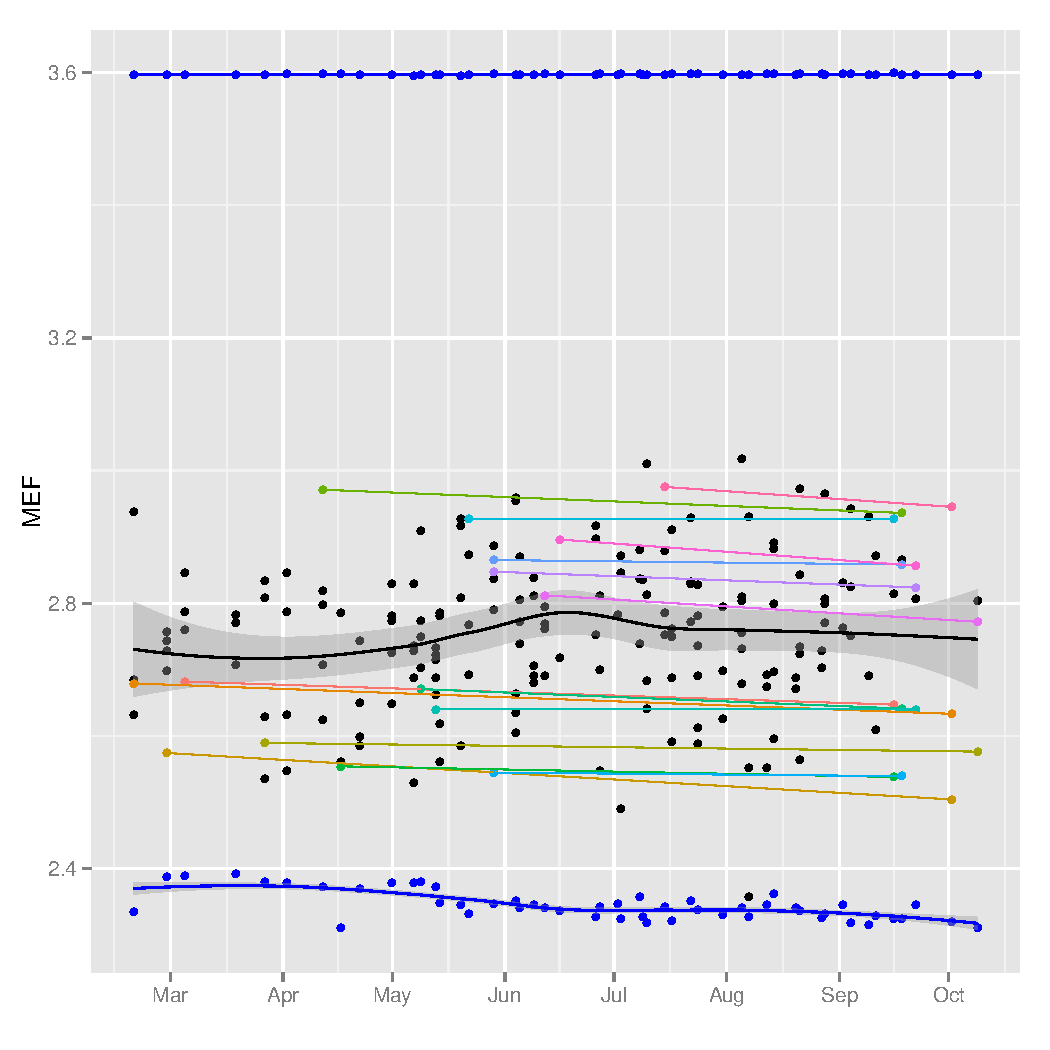
\includegraphics[scale=.5]{IL2RA/figures/CD25-MFI-time-effect-beads-normalised.pdf}
        \caption{Normalised}
    \end{subfigure}
    ~
    \begin{subfigure}[b]{.5\textwidth}
        \centering
        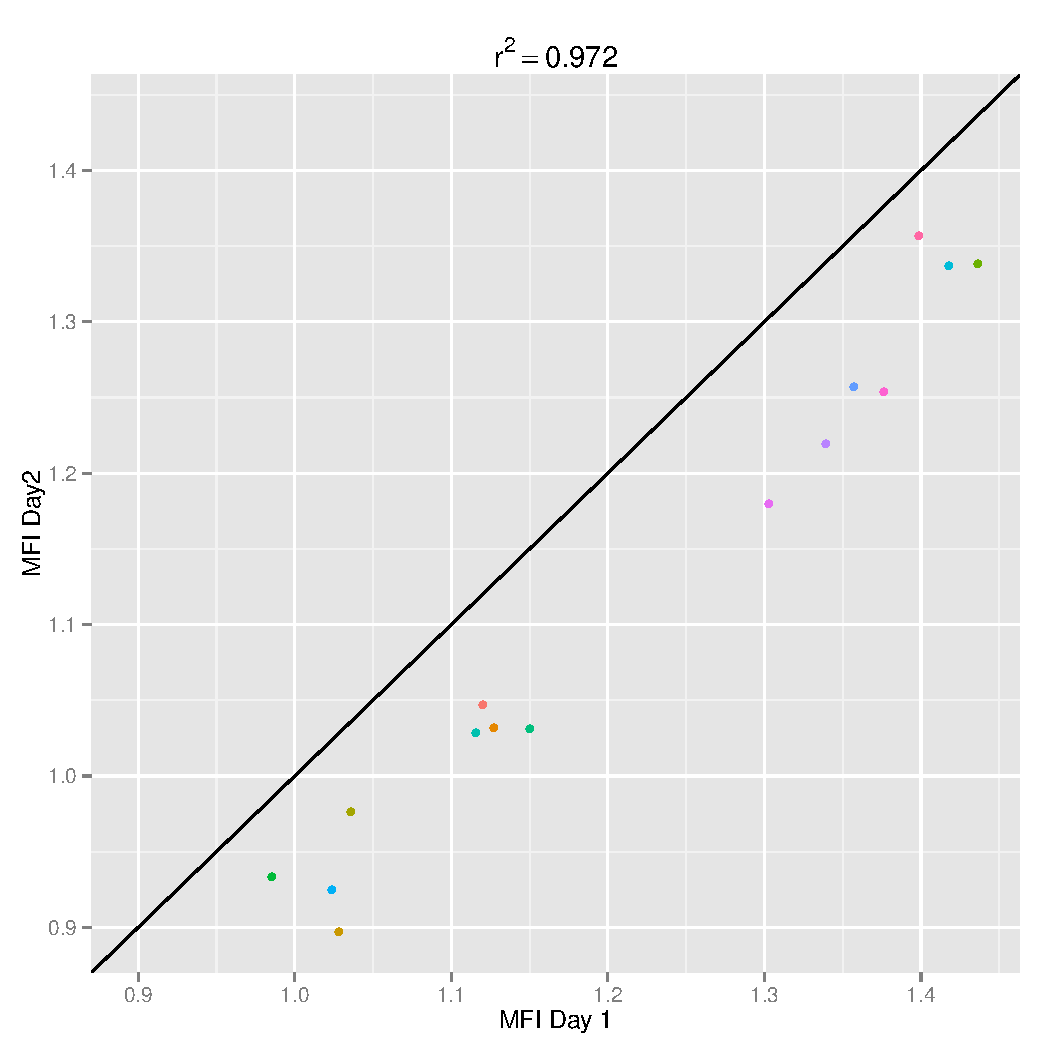
\includegraphics[scale=.75]{IL2RA/figures/CD25-MFI-repeatability.pdf}
        \caption{Unormalised: $R^2=0.629$}
    \end{subfigure}
    ~
    \begin{subfigure}[b]{.5\textwidth}
        \centering
        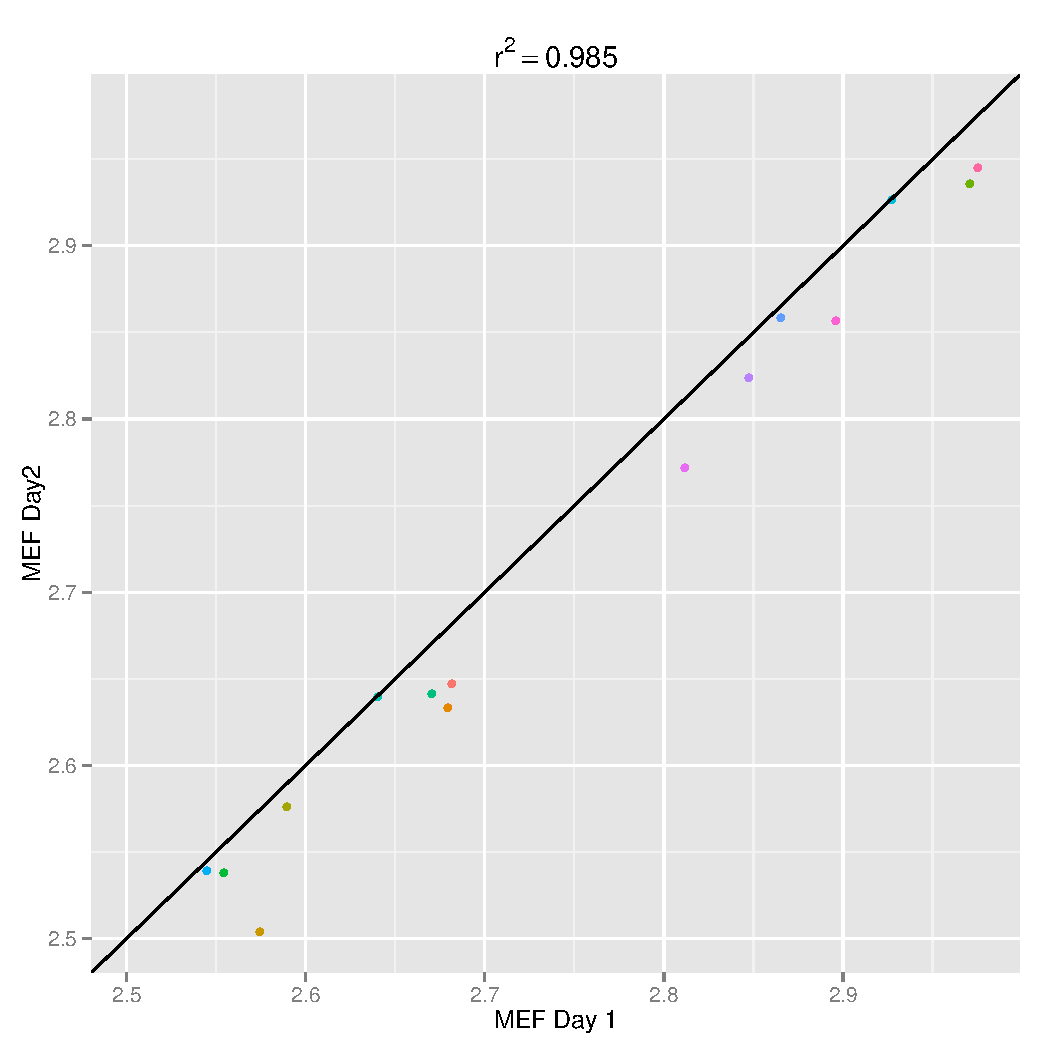
\includegraphics[scale=.75]{IL2RA/figures/CD25-MFI-beads-normalised.pdf}
        \caption{Normalised: $R^2=0.937$}
    \end{subfigure}
%\end{center}
    \caption{ \label{figure:CD25-MFI-beads-normalised.pdf}
\textbf{Bead normalisation partly corrects for long term time effect in CD25 MFI of the memory cell population.}
In \textbf{(a)} and \textbf{(b)}, the blue points represent the MFIs of the bead populations, in black the MFIs of the memory cell populations.
A loess is fitted to the MFIs of the beads and memory cells.
The points joined by lines are MFIs from recalled individuals.
The normalisation step involves aligning the peaks of the two bead populations across days to the overall mean of each of the populations (the dashed blue).
The normalisation improves the repeatability of the MFI in recalled individuals from $R^2=0.629$ \textbf{(c)} to $R^2=0.937$ \textbf{(d)}.
}
\end{figure}




